\documentclass[tikz]{standalone}
\usetikzlibrary{calc,patterns,angles,quotes}
\usepackage{pgfplots}
\pgfplotsset{compat=newest}

\pagestyle{empty}

\begin{document}
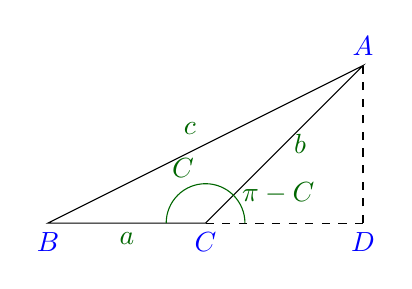
\begin{tikzpicture}
  \draw (-4,0) -- (-2, 0) -- (0, 2) -- cycle;
  \draw [blue] (-4, 0) node[anchor=north] {$B$};
  \draw [blue] (-2, 0) node[anchor=north] {$C$};
  \draw [blue] (0, 2) node[anchor=south] {$A$};
  \draw [dashed] (-2, 0) -- (0, 0);
  \draw [dashed] (0, 0) -- (0, 2);
  \draw [blue] (0, 0) node[anchor=north] {$D$};
  \draw [black!60!green] (-2, 1) node[anchor=south east] {$c$};
  \draw [black!60!green] (-3, 0) node[anchor=north] {$a$};
  \draw [black!60!green] (-1, 1) node[anchor=west] {$b$};
  \coordinate (A) at (0, 2);
  \coordinate (B) at (-4, 0);
  \coordinate (C) at (-2, 0);
  \coordinate (D) at (0, 0);
  \pic [draw, black!60!green, "$C$", angle eccentricity=1.5] {angle = A--C--B};
  \pic [draw, black!60!green, "$\pi - C$", angle eccentricity=2] {angle = D--C--A};
\end{tikzpicture}
\end{document}
